\newpage

\section{heatmap}

\begin{minipage}{.45\linewidth}
	
	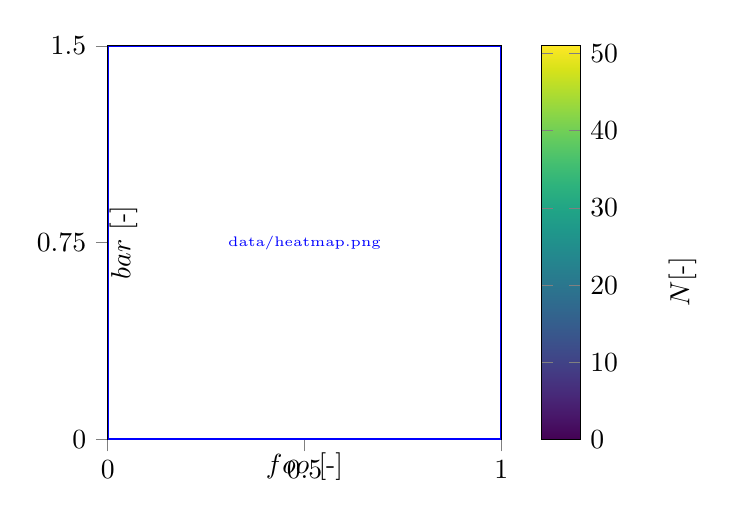
\begin{tikzpicture}
	\begin{axis}[
	scale=1,
	/pgfplots/scale only axis,
	/pgfplots/width=5cm,
	/pgfplots/height=5cm,
	colorbar,
	colorbar style={ylabel={}},
	colormap/viridis,
	point meta max=51,
	point meta min=0,
	tick align=outside,
	tick pos=left,
	xmin=0-.5, xmax=10-.5,
	ymin=0-.5, ymax=10-.5,
	xtick={-0.5,4.5,9.5},
	xticklabels={$0$,$0.5$,$1$},
	ytick={-0.5,4.5,9.5},
	yticklabels={$0$,$0.75$,$1.5$},
	x label style={at={(axis description cs:0.5,-0.01)},anchor=north},
	y label style={at={(axis description cs:+0.1,.5)},rotate=0,anchor=south},
	xlabel={$foo$ [-]},
	ylabel={$bar$ [-]},
	]
	
	\addplot graphics 
	[includegraphics cmd=\pgfimage,xmin=-0.5, xmax=9.5, ymin=9.5, ymax=-0.5] 
	{data/heatmap.png};
	
	\end{axis}
	\node at (7cm,2cm) [anchor=north , rotate=90] {$N$[-]};
	
	\end{tikzpicture}
\end{minipage}
\hfill
\begin{minipage}{.45\linewidth}
	
	\begin{tikzpicture}
	\begin{axis}[
	scale=1,
	/pgfplots/scale only axis,
	/pgfplots/width=5cm,
	/pgfplots/height=5cm,
	colorbar,
	colorbar style={ylabel={}},
	colormap/viridis,
	point meta max=3.93,
	point meta min=0,
	tick align=outside,
	tick pos=left,
	xmin=0-.5, xmax=10-.5,
	ymin=0-.5, ymax=10-.5,
	xtick={-0.5,4.5,9.5},
	xticklabels={$0$,$0.5$,$1$},
	ytick={-0.5,4.5,9.5},
	yticklabels={$0$,$0.75$,$1.5$},
	x label style={at={(axis description cs:0.5,-0.01)},anchor=north},
	y label style={at={(axis description cs:+0.1,.5)},rotate=0,anchor=south},
	xlabel={$foo$ [-]},
	ylabel={$bar$ [-]},
	]
	
	\addplot graphics 
	[includegraphics cmd=\pgfimage,xmin=-0.5, xmax=9.5, ymin=9.5, ymax=-0.5] 
	{data/heatmap_log.png};
	
	\end{axis}
	\node at (7cm,2cm) [anchor=north , rotate=90] {$\log(N)$[-]};
	
	\end{tikzpicture}
\end{minipage}


\subsection{how to}
\begin{itemize}
	\item preprocessing with python:
	\begin{itemize}
		\item import packages
	\begin{lstlisting}[language=python]
import numpy as np
import matplotlib.pyplot as plt
\end{lstlisting}
	\item transform rawdata to grid:
	\begin{lstlisting}[language=python]
def generate_grid( min, max, num ):

   cell_borders = np.linspace(min,max,num)

   def pos_in_grid(val):
      pos = sum( [1 if x <= val else 0 for x in cell_borders[1:-1] ] )
      return pos

   return pos_in_grid


def data_2_grid( filename,x_min, x_max, y_min, y_max, res_x, res_y ):

   with open(filename, "r") as fp:
      x_data, y_data = np.loadtxt(fp, 
                                  delimiter=' ',
                                  usecols=(0,1), 
                                  unpack = True)

   pos_in_x_grid = generate_grid(x_min, x_max, res_x+1)
   pos_in_y_grid = generate_grid(y_min, y_max, res_y+1)

   grid = np.zeros((res_x, res_y))

   for x,y in zip(x_data, y_data):
      j = pos_in_x_grid(x)
      i = pos_in_y_grid(y)
      grid[i][j] += 1

   return grid
	\end{lstlisting}
	\item create grid from raw data
	\begin{lstlisting}[language=python]
grid = data_2_grid("example_001.csv",0,1,0,1.5,10,10)
	\end{lstlisting}
	\item (Optional for log(N)- heatmap) filter grid :
	\begin{lstlisting}[language=python]
grid = [[ 0 if val == 0 else np.log(val) for val in row ] for row in grid]
	\end{lstlisting}

\item create image file
\begin{lstlisting}[language=python]
fig = plt.figure(frameon = False)
fig.set_size_inches(2,2)
ax = plt.Axes(fig, [0,0,1,1])
ax.set_axis_off()
fig.add_axes(ax)
ax.imshow(grid,  origin='lower')
fig.savefig("heatmap.png")
	\end{lstlisting}
	\item get information for plot configuration:
\begin{lstlisting}[language=python]
print(np.max(grid))  # point meta max
print(np.min(grid))  # point meta min 
\end{lstlisting}
	\end{itemize}

\item plot commands:

\begin{lstlisting}
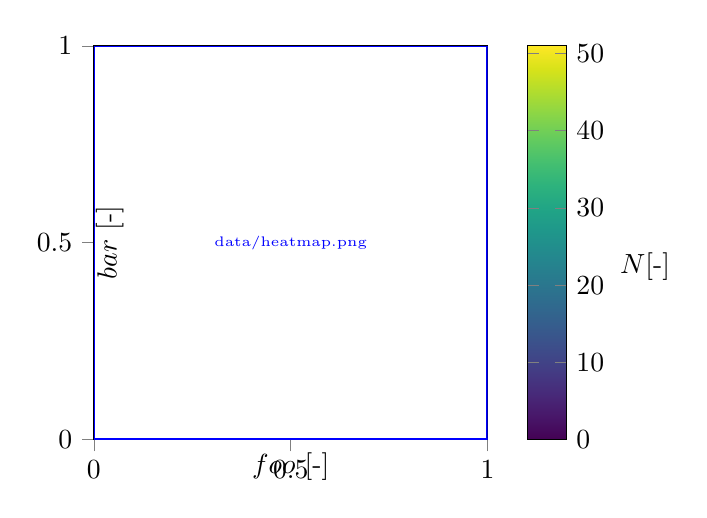
\begin{tikzpicture}
\begin{axis}[
scale=1,
/pgfplots/scale only axis,
/pgfplots/width=5cm,
/pgfplots/height=5cm,
colorbar,
colorbar style={ylabel={}},
colormap/viridis,
point meta max=51,  % max value from grid data in python
point meta min=0,  % min value from grid data in python
tick align=outside,
tick pos=left,
xmin=0-.5, xmax=10-.5,
ymin=0-.5, ymax=10-.5,
xtick={-0.5,4.5,9.5},
xticklabels={$0$,$0.5$,$1$},
ytick={-0.5,4.5,9.5},
yticklabels={$0$,$0.5$,$1$},
x label style={at={(axis description cs:0.5,-0.01)},anchor=north},
y label style={at={(axis description cs:+0.1,.5)},rotate=0,anchor=south},
xlabel={$foo$ [-]},
ylabel={$bar$ [-]},
]

\addplot graphics 
[includegraphics cmd=\pgfimage,xmin=-0.5, xmax=9.5, ymin=9.5, ymax=-0.5] 
{data/heatmap.png};

\end{axis}

\node at (7cm,2.5cm) [anchor=north , rotate=0] {$N$[-]};

\end{tikzpicture}
\end{lstlisting}

\end{itemize}

